\chapter{Chapitre 1 : État de l'art} % Main chapter title

\label{Chapter1} % For referencing the chapter elsewhere, use \ref{Chapter1} 

%----------------------------------------------------------------------------------------

\section{Introduction}
La détection et le suivi de cibles englobent une large variété de problèmes décisionnels, tels que la surveillance, la recherche, les patrouilles, l’observation et la poursuite-évasion. Compte tenu du besoin croissant en effectif, en temps et en minimisation des coûts, de nombreuses applications ont été développées notamment dans des domaines comme le commerce et la défense.

Dans ce chapitre, nous nous attelons à fournir une synthèse sur les différents travaux inhérents à la recherche de multiples cibles dans un environnement inconnu et complexe. Au préalable, nous devons introduire certaines définitions et techniques propres à la nature des environnements auxquels nous aurons à faire face, d’autres concernant les méthodes de résolution. On finira par une conclusion dans laquelle nous situerons clairement la problématique traitée. 



\section{Problématique} 
\textbf{Pourquoi s'intéresser à la détection de cibles ?}\\

La détection de cibles est un problème intéressent dont la résolution apporte des avantages et gain de temps couvrant diverses besoins quotidiens qui s'étalent sur divers domaines.

Nous nous intéressons particulièrement à la recherche de mines anti-personnelles et bombes ainsi que la recherche de sources radioactives, car rien n’est plus important que la sécurité et la mise hors de danger de vies humaines.

Pour cela, nous aurons recours à des méthodes de résolution basées sur l’intelligence en essaim. Ces méthodes ont permis dernièrement de maintes avancées, jugées les plus adéquates comme technique de résolution.

De ce fait, nous aurons besoin de développer un système multi-robots où chaque robot se comportera comme une particule de l’essaim.

L’environnement inconnu est considéré en 2D, chaque robot n’a connaissance que du nombre de cibles recherchées, les bordures ou frontières de l’environnement de recherche ainsi que sa position initiale (position avant le début de la recherche).
Aussi l’environnement est complexe et englobe plusieurs obstacles, entravant son exploration.

Les positions des obstacles sont inconnues, c’est pourquoi les robots doivent être munis de capteurs adaptés à leur stratégie d’évitement d’obstacles.
Les cibles (mines / sources de radiation) dont les positions sont inconnues, émettent un signal que les robots sont capables de réceptionner via leurs capteurs.

La validation du système sera effectuée par des expérimentations sur des environnements dont les positions des obstacles, cibles et des robots sont générées aléatoirement. Cela conformément à la procédure présentée dans des travaux récents.





\section{Paramètres du problème}
Plusieurs paramètres entrent en jeu concernant le problème de recherche de cibles, donnant lieu à une arborescence de sous-classes de problèmes (voir figure \ref{classesProb}), qui se diffèrent par les techniques de résolutions adaptées.

\begin{center}	  
	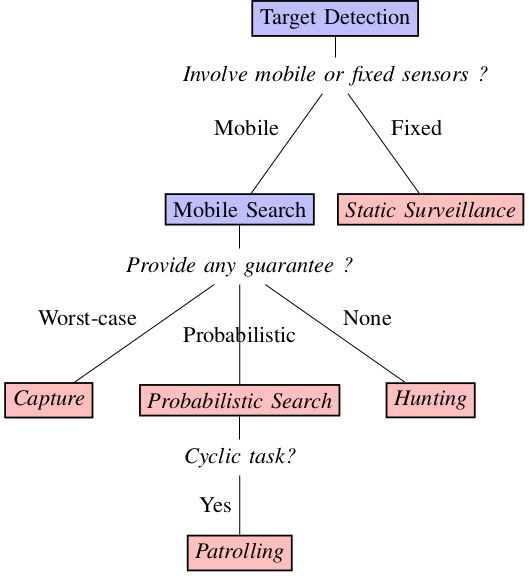
\includegraphics[width=0.4\textwidth]{../Figures/targetdetection.png}%
	\vspace{-0.1 cm}
	\captionof{figure}{Schéma résumant les classes de problèmes de détection de cibles \cite{surv2}.}\label{classesProb}%
\end{center}

Nous distinguons quatre types de problèmes : 
\begin{itemize}
	\item[$\bullet$] \textbf{La surveillance statique} implique l’utilisation de robots fixes dans un environnement connu afin d’entièrement le couvrir pour y détecter les cibles \cite{surv2}. 
	
	
	
	\item[$\bullet$] \textbf{La capture} a pour but de capturer toutes les cibles présentes dans un environnement connu. Seules les positions initiales des cibles ne sont pas connues par le(s) poursuiveur(s) \cite{surv2}. La figure \ref{capture} illustre un exemple de capture.
	\begin{center}	  
		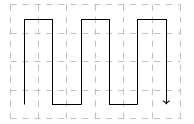
\includegraphics[width=0.27\textwidth]{../Figures/capture.png}%
		\vspace{-0.1 cm}
		\captionof{figure}{Exemple de capture \cite{surv2}.}\label{capture}%
	\end{center}
	
	
	
	\item[$\bullet$] \textbf{La patrouille} a une formulation proche de celle de capture, mais avec un aspect cyclique. Autrement dit la zone n’est pas couverte qu’une seule fois, mais plusieurs fois \cite{surv2}, comme le montre la figure \ref{patrou}.
	\begin{center}	  
		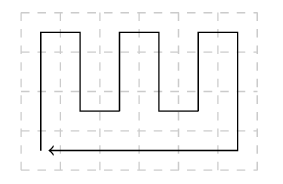
\includegraphics[width=0.3\textwidth]{../Figures/patrolling.png}%
		\vspace{-0.1 cm}
		\captionof{figure}{Exemple de patrouille \cite{surv2}.}\label{patrou}%
	\end{center}
	
	\item[$\bullet$] \textbf{La chasse} s’attaque à la détection de cibles sans aucune garantie. C’est-à-dire qu’on suppose qu’on ne connaît ni les positions initiales des cibles ni l’environnement de recherche \cite{surv2}. \\
\end{itemize}



À partir de la formulation de la problématique et des classes de problèmes présentées ci-dessus, on peut clairement situer notre contribution, qui s'inscrit dans le cadre des problèmes de type  \textbf{Chasse}. 

Dans ce qui suit nous dériverons les paramètres du problème les plus pertinents :


\subsection{Les systèmes multi-robots (SMRs)}

\subsubsection{Définition}
Un système multi-robots est un groupe de robots mobiles autonomes ayant un objectif ou un ensemble de tâches communes, ces robots ont la capacité de communiquer et se coordonner afin d'atteindre leur objectif \cite{SMR1}. 

Les robots mobiles se déplacent durant la recherche selon une stratégie visant à aboutir à des solutions optimales.

Il est important de souligner que le mode de mobilité des robots influence fortement la résolution du problème (vision, vitesse, agilité du mouvement) \cite{surv1}.



\subsubsection{Caractéristiques des SMRs \cite{surv1}}
Les systèmes multi-robots se caractérisent par multiples aspects qui font leur force, à commencer par l'exécution des tâches en parallèle, ainsi qu’une couverture d'une plage assez importante de l'espace de recherche. D'autres particularités des SMRs spécifiques aux essaims de robots existent, telles que:
\begin{itemize}
	\item[$\bullet$]\textit{La robustesse}, qui offre une tolérance aux pannes.
	
	\item[$\bullet$]\textit{la flexibilité} permet une rapide adaptation aux nouvelles exigences et différents environnements (favorisée par la redondance et la simplicité des comportements des robots).
	
	\item[$\bullet$]\textit{l'évolutivité} qui est la capacité à fonctionner avec un nombre plus grand ou plus petit de robots sans impact considérable sur la performance.
\end{itemize}

\subsubsection{Système de communication \cite{surv2}}
Deux types de systèmes sont les plus répandus: centralisés et décentralisés, ils sont choisis selon le besoin et les critères recherchés.


\begin{itemize}  
	\item[$\bullet$] \textbf{Les systèmes centralisés}, sont plus aptes à fournir une optimalité globale. Cependant, ils sont souvent confrontés à de fortes contraintes du  monde réel, d’où la nécessité d'une connectivité totale dans de nombreuses situations.
	
	\item[$\bullet$] \textbf{Les systèmes décentralisés}, quant à eux fournissent des solutions jugées sous-optimales. Par contre, ils sont plus robustes et plus flexibles de par leur adaptation aux environnements dynamiques ce qui leur permet d'aboutir à des performances intéressantes.
\end{itemize}


\subsubsection{Comportement des robots \cite{surv2}}
Les robots peuvent s'approprier deux types de comportements, soient:

\begin{itemize} 
	\item[$\bullet$] \textbf{Indépendant}, chaque robot est responsable d'un certain nombre de tâches à exécuter.
	
	\item[$\bullet$] \textbf{Coopératif}, chaque décision ou action est diffusée à toute l'équipe. Ce mode coopératif peut être explicite, consistant à influencer un robot par une communication directe, ou bien implicite, qui est une  prise de décision indépendante selon les informations individuellement recueillies.
\end{itemize}


\subsection{Les capteurs}
Selon l'environnement à explorer, le besoin en types de capteurs diffère, que ce soit pour reconnaître les cibles, détecter les obstacles afin de les éviter ou reconnaître les autres robots.

Parmi la panoplie des capteurs existants, on trouve : les caméras, les infrarouges, les capteurs lasers (distance), les capteurs à ultrason, la kinect, les capteurs de pression, les capteurs de gaz, GPS, ...etc \cite{capteur} qui sont les plus utilisés. Le choix des capteurs consiste à trouver le meilleur compromis entre coût et efficacité selon les contraintes imposées. 

\subsection{Les cibles}
Le nombre de cibles est un paramètre fixé pour un environnement donné. Les problèmes \textbf{mono-cible} consistent à trouver la position d'une cible particulière dans l'environnement. En revanche, les problèmes \textbf{multi-cibles} visent à maximiser le nombre de cibles trouvées. 

Pour le problème de recherche ou détection, les cibles possèdent des positions inchangées dans l'environnement durant toute la recherche 
\cite{surv1}.\\

De plus, il est toujours supposé que les cibles émettent des radiations, sons, ondes, lumières, odeurs ou autres, qui sont maximales aux alentours de la cible  s'estompant graduellement en s'éloignant de celle-ci. L'étendue du champ d'émission de ces cibles est aussi un paramètre qui influe directement l'efficacité des algorithmes de résolution.

\subsection{L'environnement \cite{surv2}}
L'environnement est l'espace de recherche où évoluent les cibles et interviennent les robots comme fouilleurs. Il est décrit comme \textbf{connu} lorsqu’une carte est mise à disposition et \textbf{inconnu} lorsqu'on manque d'informations globales, n'ayant connaissance que de ses bordures. Ces environnements peuvent être des:

\begin{itemize} 
	\item[$\bullet$] \textbf{Environnements simples}, c'est-à-dire sans obstacles ne contenant aucune contrainte susceptible de bloquer la vue ou la mobilité des robots.
	
	\item[$\bullet$] \textbf{Environnements avec obstacles ou complexes}, Ceux-ci contenant des obstacles, contraignants ainsi les robots dans leurs déplacements et leurs perceptions, les poussant parfois à changer de trajectoire.
\end{itemize}

\subsection{Les obstacles}
Les obstacles sont des contraintes supplémentaires dans le processus de recherche de cibles. Divers types d'obstacles existent, citons les obstacles fixes et mobiles, les obstacles franchissables mais entravant la vue ou encore les obstacles empêchant uniquement le passage sans obstruer la visibilité des robots, ... etc \cite{surv2}.\\

La présence d'obstacles dans les environnements de recherche impose aux méthodes de résolution une prise en considération d'une stratégie d'évitement d'obstacles, pour cela nombreuses sont les stratégies existantes.

Elles s'appuient sur les informations fournies par les capteurs embarqués afin d'orienter les robots à chaque laps de temps pour une réaction en temps réel \cite{Sara}. 





%\newpage


\section{Travaux connexes}
Plusieurs approches ont été exploitées pour la résolution du problème de détection de cibles dans des environnements inconnus, nous citons à titre d'exemple:

\subsection{Les algorithmes anti-regroupements \cite{Miao2010}}
Souvent appliqués aux problèmes de type "chasse", ces algorithmes imitent le comportement social des animaux solitaires (tigre, araignée, ...). Ils se basent sur trois principales règles, soient:

\begin{itemize}
	\item[$\bullet$] La prévention des collisions : en s'éloignant des obstacles les plus proches et en respectant une distance de sécurité.
	
	\item[$\bullet$] La décentralisation : en tentant de se séparer de ses voisins.
	
	\item[$\bullet$] L'égoïsme : si aucune des deux situations précédentes ne se produit, chaque robot choisit la direction permettant de maximiser ses propres gains.
\end{itemize}


\subsection{Approche des champs de potentiel \cite{surv2}}
Dans cette approche on considère deux vecteurs de forces locales qui influencent les mouvements des robots telles que, les cibles proches émettent des forces attractives vers elles, tandis que les robots proches émettent des forces répulsives éloignant ainsi les autres robots. L'algorithme de Parker pour le contrôle distribué A-CMOMMT est inspiré des champs de potentiels \cite{Parker2002}.

\subsection{Approches basées intelligence en essaim}
L'intelligence  en essaim  et les méta-heuristiques ont été très exploitées pour ce type de problème grâce à la facilité des opérations stochastiques qui les distinguent des autres techniques. Leur force majeure est l'inspiration des  comportements d'espèces ou phénomènes naturels \cite{robotMeta}.\\

PSO, GA, ACO, BA, ABC, BFO, GSO et FA sont les techniques de méta-heuristiques les plus utilisées revenant souvent dans la littérature avec des améliorations et contributions apportées par les auteurs \cite{surv1}. 

Quant aux travaux récents on trouve :

\subsubsection{BSO (Bee Swarm Optimization) (2013)}
Une variante de l’algorithme Bee Swarm Optimization inspirée du comportement des abeilles dont les auteurs sont Hannaneh Najd Ataei, Koorush Ziarati et Mohammad Eghtesad \cite{BSO2013} comporte trois types d’abeilles (abeilles butineuses, abeilles éclaireuses, abeilles spectatrices) chacune possède sa propre fonction de mise à jour de ses positions.\\	

Cette variante a montré de meilleures performances que la version classique de PSO.
Suite à des expérimentations sur un ensemble d’environnements aléatoires, il a été prouvé que cette approche de BSO peut être 50,6\% plus efficace que PSO.

Mais elle n’a été testée que sur des environnements mono-cibles. De plus, la fonction objectif utilisée s’appuie sur  la distance euclidienne entre les robots et la cible, or que les positions des cibles sont supposées inconnues.

\subsubsection{A-RPSO}
A-RPSO (Adaptative Robotic Particule Swarm Optimization) est une technique basée essaim proposée par les auteurs M. Dadgar, et al., où chaque particule représente un robot. La contribution de l’auteur par rapport à un PSO classique est l’ajout d’une stratégie d’évitement d’obstacles incluse dans l’équation de déplacement, ainsi qu’une mise à jour des paramètres classiquement constants comme le poids d'inertie de façon dynamique,  dite adaptative.\cite{Dadgar2016}.



Ces modifications ont eu comme objectif d’éviter les optimaux locaux, mieux contrôler et adapter l’allure des robots lors du rapprochement des cibles et des obstacles. La technique a été testée sur un simulateur 2D créé par les auteurs, elle reste proche d’une modélisation d’une grille virtuelle bidimensionnelle.  


\subsubsection{MFSO (Multi-swarm hybrid FOA-PSO)}
Un nouvel algorithme multi-essaim hybride (MFPSO) basé sur FOA (Fruit Fly Optimization Algorithm) et PSO (Particule Swarm Optimization) pour la recherche d’une cible dans des environnements inconnus a été présenté par les auteurs, Hongwei Tang, Wei Sun, Hongshan Yu, Anping Lin, Min Xue et Yuxue Song \cite{novel}. Cette nouvelle méta-heuristique se singularise par les avantages suivants : \\

\begin{itemize}
	\item [$\bullet$] Parallélisme grâce à un coefficient adaptatif.
	
	\item[$\bullet$] Présence de stratégies contournant la convergence prématurée grâce à l'indépendance des essaims de robots.
	
	\item[$\bullet$] Mécanisme d'évacuation (MSCM) comme stratégie d'évitement d'obstacles.\\
\end{itemize}

Les nombreuses expériences effectuées pour le mode mono-cible sur MFPSO prouvent qu’il surpasse de manière significative les autres approches (dont A-RPSO et RPSO), en termes de nombre d’itérations et taux de réussite, dans la plupart des cas.
 
Par contre, le champ d’émission de la cible est inconnu, or comme mentionné plus haut, ce paramètre influence la difficulté du problème.
 
Les tests effectués comportent le cas du mono-cible seulement, ce qui implique que le comportement et l’efficacité de cet algorithme dans des environnements multi-cibles sont inconnus. 

Aussi, le champ de vue des robots a été fixé par les auteurs à une valeur de dix pixels durant toutes les expérimentations. 

Enfin, les auteurs utilisent une fonction objectif qui manipule la distance $ Dist \left( x^{t}_{i} \right)$ entre les robots et la cible. Cependant, la position de la cible est supposée inconnue. C’est pourquoi cette distance au lieu d’être directement utilisée comme fonction objectif elle a servi à calculer une estimation des signaux émis par la cible. 





\section{Conclusion}
Ce chapitre nous a permis de décortiquer les différentes variantes du problème de détection de cibles ce qui nous a permis de déduire que notre travail visera à proposer une solution au problème de \textit{Chasse}.

 Tous les paramètres nécessaires pour clairement définir notre problème et aboutir à une bonne modélisation, ont été explicitement exposés.
Notre méthode de résolution est basée intelligence en essaim, d’où la nécessité d'éclaircir certains aspects incontournables relatifs aux approches choisies dans le chapitre suivant.
